\documentclass[11pt]{article}
\usepackage[a4paper,margin=1in]{geometry}
\usepackage{amsmath,amssymb,amsthm}
\usepackage{graphicx}
\usepackage[hidelinks]{hyperref}
\setlength{\emergencystretch}{3em}

\newtheorem{theorem}{Theorem}
\newtheorem{remark}{Remark}
\DeclareMathOperator*{\argmin}{arg\,min}
\newcommand{\crit}{\operatorname{crit}}
\newcommand{\Rbar}{\overline{\mathbb R}}

\title{A Two-Datum Obstruction to Representing Relative-Critical\\
Sets by a Data-Independent Tikhonov Regularizer}
\author{Automatic math-discovery packet}
\date{August 11, 2026}

\begin{document}
\maketitle

\section*{Source Conjecture}

The source is Daniel Obmann and Markus Haltmeier,
\emph{Convergence analysis of critical point regularization with non-convex
regularizers}, arXiv:2207.14480v2 \cite{OH2023}. In Section~4.3, pages 19--20,
the authors ask whether their regularization by \(\alpha\phi\)-critical points
can be equivalent to ordinary Tikhonov regularization with a modified penalty
\(\mathcal R_\phi\). They conjecture:

\begin{quote}
``the proposed regularization is not equivalent to Tikhonov regularization
independent of the choice \(\mathcal R_\phi\).''
\end{quote}

The source discussion makes this a set-valued comparison: the full set of
\(\alpha\phi\)-critical points is to coincide with the full minimizer set of a
Tikhonov functional using one modified regularizer independent of the datum.
The complete source passage spans the following two crops.

\begin{figure}[htbp]
\centering
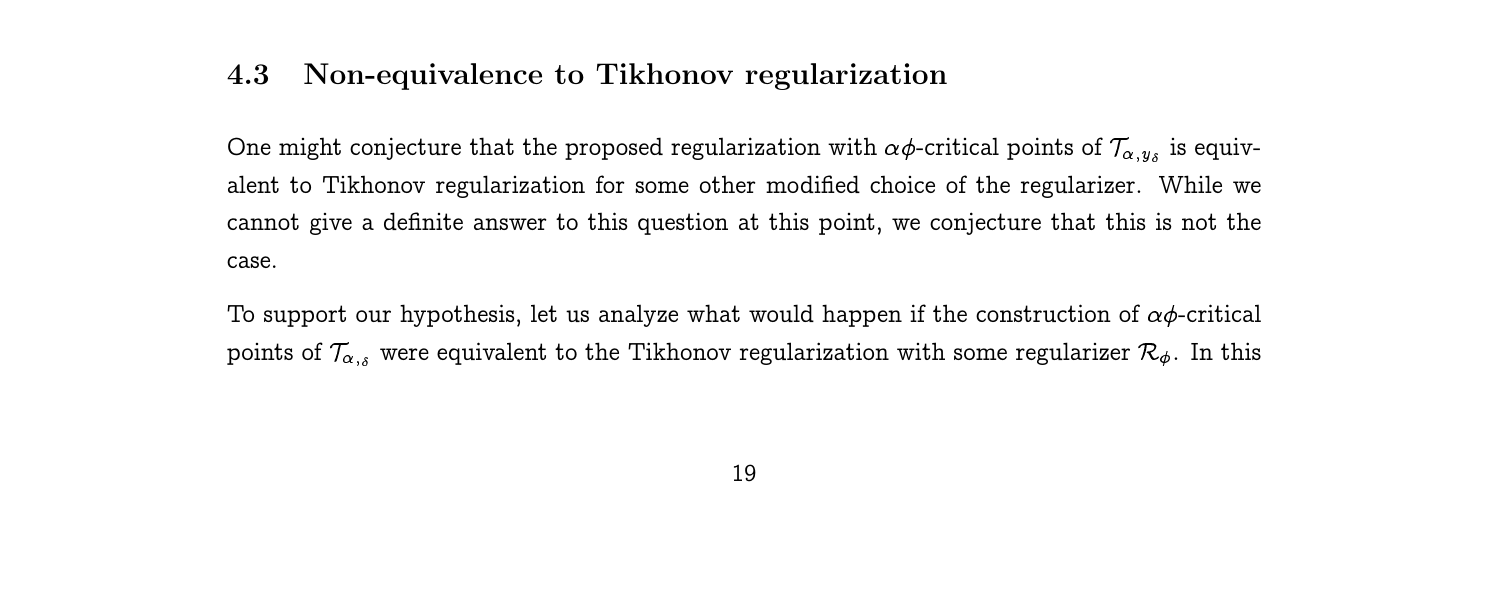
\includegraphics[width=\textwidth]{figures/open_problem_crop_page19.png}
\vspace{0.5em}

\includegraphics[width=\textwidth]{figures/open_problem_crop_page20.png}
\caption{Section 4.3 of the source paper, pages 19--20.}
\end{figure}

\section*{Definitions}

For a function \(F:X\to\mathbb R\) and a bound
\(\psi:X\to[0,\infty)\), the source defines
\(r\in\partial_\psi F(x)\) by
\[
 F(x)+\langle r,u-x\rangle\leq F(u)+\psi(u)
 \qquad (u\in X).
\]
The point \(x\) is \(\psi\)-critical if
\(0\in\partial_\psi F(x)\). Consequently,
\begin{equation}
\label{eq:critical-sublevel}
 x\in\crit_\psi F
 \quad\Longleftrightarrow\quad
 F(x)\leq\inf_{u\in X}\bigl(F(u)+\psi(u)\bigr).
\end{equation}
This is also Lemma~2.4(6) of the source paper.

For data \(y\in Y\), a linear forward map \(K:X\to Y\), a penalty
\(\mathcal R\), and \(\alpha>0\), the Tikhonov functional is
\[
 \mathcal T_{\alpha,y}(x)
 =\frac12\lVert Kx-y\rVert^2+\alpha\mathcal R(x).
\]
An ordinary modified-penalty representation of its relative-critical sets
would be a proper function \(S:X\to(-\infty,+\infty]\), independent of \(y\),
such that
\[
 \crit_{\alpha\phi}\mathcal T_{\alpha,y}
 =\argmin_x\left\{\frac12\lVert Kx-y\rVert^2+\alpha S(x)\right\}
\]
for all data under consideration.

\clearpage
\section*{Proof Intuition}

It is enough to use the most elementary admissible instance of the source
framework: one dimension, identity forward map, zero original regularizer, and
a positive constant relative-error bound. Formula
\eqref{eq:critical-sublevel} then turns the relative-critical set into a closed
interval of fixed positive radius centered at the datum.

Two nearby data give two overlapping intervals. Choose their two centers so
that both centers lie in both intervals. If one data-independent penalty made
both intervals minimizer sets, then the modified Tikhonov objective would have
equal values at the two centers for each datum. Moving the quadratic data term
from one center to the other reverses its sign, forcing the same penalty
difference to equal both \(\varepsilon\) and \(-\varepsilon\). This is the
desired obstruction.

\section*{Main Theorem}

\begin{theorem}[No data-independent modified penalty]
\label{thm:main}
Fix \(\alpha>0\) and \(\varepsilon>0\). Let
\[
 X=Y=\mathbb R,\qquad K=I,\qquad \mathcal R\equiv0,
 \qquad \phi\equiv\varepsilon,
\]
and put \(\rho=\sqrt{2\alpha\varepsilon}\). Then for every \(y\in\mathbb R\),
\[
 \crit_{\alpha\phi}\mathcal T_{\alpha,y}
 =[y-\rho,y+\rho].
\]
There is no proper function \(S:\mathbb R\to(-\infty,+\infty]\) for which
\begin{equation}
\label{eq:representation}
 \argmin_{x\in\mathbb R}
 \left\{\frac12(x-y)^2+\alpha S(x)\right\}
 =\crit_{\alpha\phi}\mathcal T_{\alpha,y}
\end{equation}
holds for every \(y\in\mathbb R\). In fact, no such \(S\) can make
\eqref{eq:representation} hold simultaneously for the two data values
\(y=0\) and \(y=\rho\).
\end{theorem}

\begin{proof}
Here
\[
 \mathcal T_{\alpha,y}(x)=\frac12(x-y)^2
 \quad\text{and}\quad
 \inf_u\bigl(\mathcal T_{\alpha,y}(u)+\alpha\phi(u)\bigr)
 =\alpha\varepsilon.
\]
Therefore \eqref{eq:critical-sublevel} gives
\[
 x\in\crit_{\alpha\phi}\mathcal T_{\alpha,y}
 \quad\Longleftrightarrow\quad
 \frac12(x-y)^2\leq\alpha\varepsilon
 \quad\Longleftrightarrow\quad
 x\in[y-\rho,y+\rho].
\]

Suppose that a proper \(S\) represents the relative-critical sets for
\(y=0\) and \(y=\rho\). Both points \(0\) and \(\rho\) belong to both relevant
intervals:
\[
 0,\rho\in[-\rho,\rho]
 \quad\text{and}\quad
 0,\rho\in[0,2\rho].
\]
Hence both are global minimizers of the modified Tikhonov objective for each
of the two data. Since \(S\) is proper, the corresponding minimum values are
finite. Equality of the values at \(0\) and \(\rho\) for datum \(y=0\) gives
\[
 \alpha S(0)=\frac12\rho^2+\alpha S(\rho),
 \qquad\text{so}\qquad
 S(0)-S(\rho)=\frac{\rho^2}{2\alpha}=\varepsilon.
\]
For datum \(y=\rho\), equality at the same two minimizers gives
\[
 \frac12\rho^2+\alpha S(0)=\alpha S(\rho),
 \qquad\text{so}\qquad
 S(\rho)-S(0)=\varepsilon.
\]
Adding the last two identities yields \(0=2\varepsilon\), contradicting
\(\varepsilon>0\). Thus no data-independent modified penalty exists.
\end{proof}

\begin{remark}[Strength of the obstruction]
No convexity, continuity, lower semicontinuity, or coercivity is assumed of
\(S\). The contradiction also fixes \(\alpha\), so allowing the modified
penalty to depend on \(\alpha\), on \(\varepsilon\), or on the original
regularizer does not help. Dependence on the datum is the only excluded
dependence, exactly as in the source conjecture.
\end{remark}

\section*{Verification Notes}

The proof uses only the definition of relative criticality and equality of an
objective at two global minimizers. The accompanying script
\texttt{code/verify\_two\_data\_obstruction.py} checks, for several positive
\((\alpha,\varepsilon)\) pairs, that the two selected points lie in both
relative-critical intervals and that the two minimizer equalities demand
opposite penalty differences \(\varepsilon\) and \(-\varepsilon\). Running
\begin{quote}
\texttt{python code/verify\_two\_data\_obstruction.py}
\end{quote}
prints \texttt{all checks passed}. These finite checks are only a sanity test;
the symbolic argument above proves the theorem for every
\(\alpha,\varepsilon>0\).

\section*{Limitations and Novelty Check}

The theorem settles the set-valued comparison made in Section~4.3: it shows
that critical-point regularization cannot \emph{in general} be recast as
ordinary Tikhonov minimization with a data-independent penalty. It does not
claim that every single-valued algorithmic selection from a relative-critical
set is non-Tikhonov. In this example, for instance, the selection \(x(y)=y\)
is represented by the zero penalty even though the entire interval-valued map
is not.

The run's lightweight registry, solution, attempt, and proof-gap indexes were
searched for arXiv:2207.14480 and the core equivalence terminology. Exact
queries of the official arXiv API on August 11, 2026 for ``critical point
regularization'' and ``relative sub-differentiability'' found the source, the
authors' later convergence-rates paper \cite{O2023}, and an unrelated paper on
another relative-subdifferential notion. The later follow-up does not discuss
or settle the equivalence conjecture. No arXiv answer was found within these
bounded exact-query searches.

\section*{Human Review Recommendation}

Verify that the source's word ``equivalent'' is intended in the set-valued
sense made explicit by its displayed biconditional and its discussion of the
whole set of \(\alpha\phi\)-critical points. Under that interpretation, the
example satisfies the paper's standing regularization assumptions:
\(\mathcal R=0\) is nonnegative and weakly lower semicontinuous,
\(\mathcal T_{\alpha,y}\) is coercive because \(K=I\), and the constant
\(\phi=\varepsilon\) is an admissible relative bound.

\begin{thebibliography}{9}
\bibitem{OH2023}
D. Obmann and M. Haltmeier,
\emph{Convergence analysis of critical point regularization with non-convex
regularizers}, Inverse Problems 39 (2023), 095002;
arXiv:2207.14480v2.

\bibitem{O2023}
D. Obmann,
\emph{Convergence rates for critical point regularization},
arXiv:2302.08830 (2023).
\end{thebibliography}

\end{document}

